%%%%%%%%%%%%%%%%%%%%%%%%%%%%%%%%%%%%%%%%%
% University/School Laboratory Report
% LaTeX Template
% Version 4.0 (March 21, 2022)
%
% This template originates from:
% https://www.LaTeXTemplates.com
%
%%%%%%%%%%%%%%%%%%%%%%%%%%%%%%%%%%%%%%%%%

%----------------------------------------------------------------------------------------
%	PACKAGES AND DOCUMENT CONFIGURATIONS
%----------------------------------------------------------------------------------------

\documentclass[
	a4paper, % Paper size, specify a4paper (A4) or letterpaper (US letter)
	10pt, % Default font size, specify 10pt, 11pt or 12pt
]{CSUniSchoolLabReport}

\addbibresource{sample.bib} % Bibliography file (located in the same folder as the template)
\usepackage{listings}
%----------------------------------------------------------------------------------------
%	REPORT INFORMATION
%----------------------------------------------------------------------------------------

\title{Report 5: Quantum Monte Carlo} % Report title
\subtitle{Git: https://github.com/simonblaue/MCP-Ex5.git}

\author{Simon \textsc{Blaue}} % Author name(s), add additional authors like: '\& James \textsc{Smith}'


\date{\today} % Date of the report

%----------------------------------------------------------------------------------------

\begin{document}

\maketitle % Insert the title, author and date using the information specified above

\vspace*{40px}

\begin{tabular}{l r}
	Universität Göttingen \\ % Date the experiment was performed
	Faculty of Physics \\
	Instructor: Prof. Dr. S. Schumann \\
	Tutors: Dr. E. Bothmann, M. Knobbe \\ % Partner names
\end{tabular}


% If you need to include an abstract, uncomment the lines below
%\begin{abstract}
%	Abstract text
%\end{abstract}

\newpage
%----------------------------------------------------------------------------------------
%	CONTENT
%----------------------------------------------------------------------------------------
% \headtopline
% \headsepline

\ohead{\pagemark}
\automark{subsection}

\section{Variational Monte Carlo simulation of a Helium atom}

\subsection{Investigate stepsize $s$}

First we should investiget the step size $a$, to take the smallest std. error, not influenced by the trial wave function per se. I find, that for $s=1$ I get an order of magnitude smaller std error compared to $s=0.1, 10$. Hence I will use $s=1$ for all other simulations. The results are plotted in \autoref{fig:find_a}.

\begin{figure}[H]
	\begin{subfigure}[b]{0.49\textwidth}
		\centering
		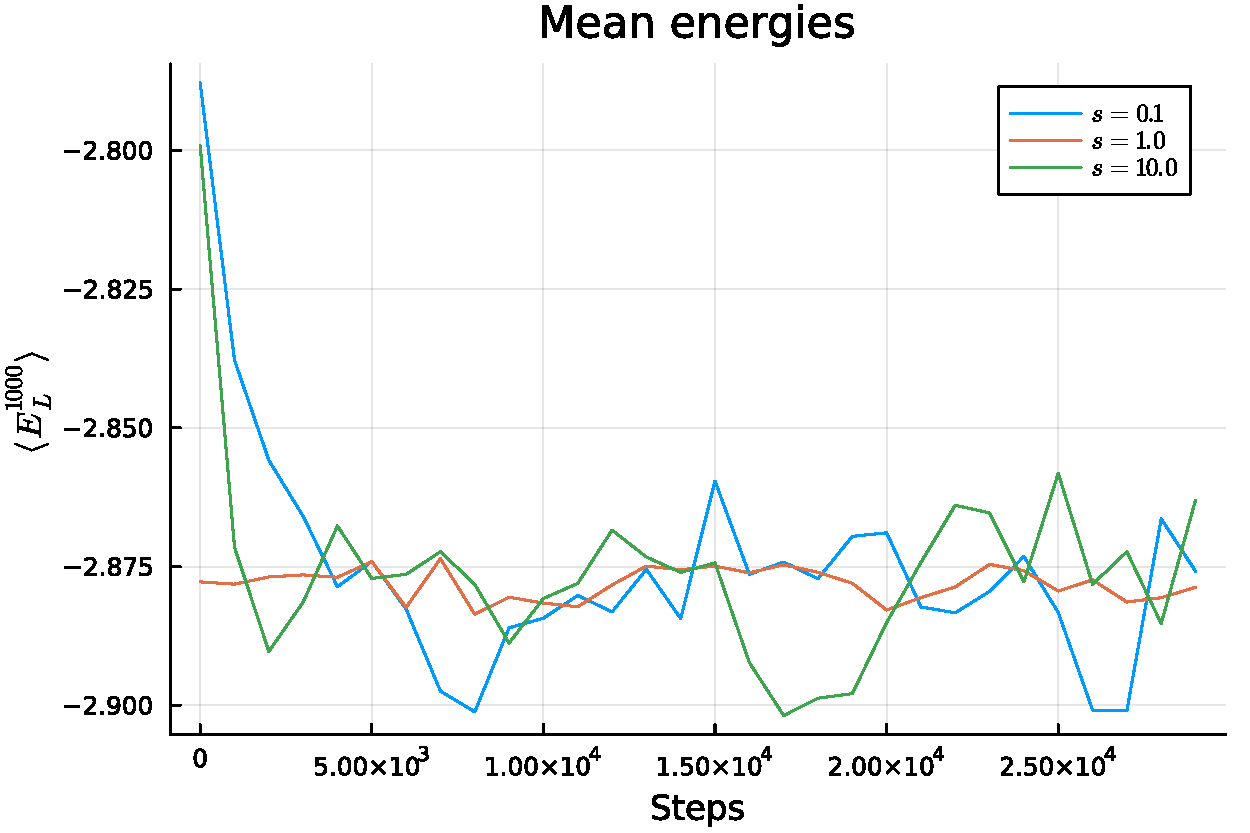
\includegraphics[width=\textwidth]{../saves/task1a.energies.pdf}
		\caption{Energies}
		% \label{fig:three sin x}
	\end{subfigure}
	\hfill
	\begin{subfigure}[b]{0.49\textwidth}
		\centering
		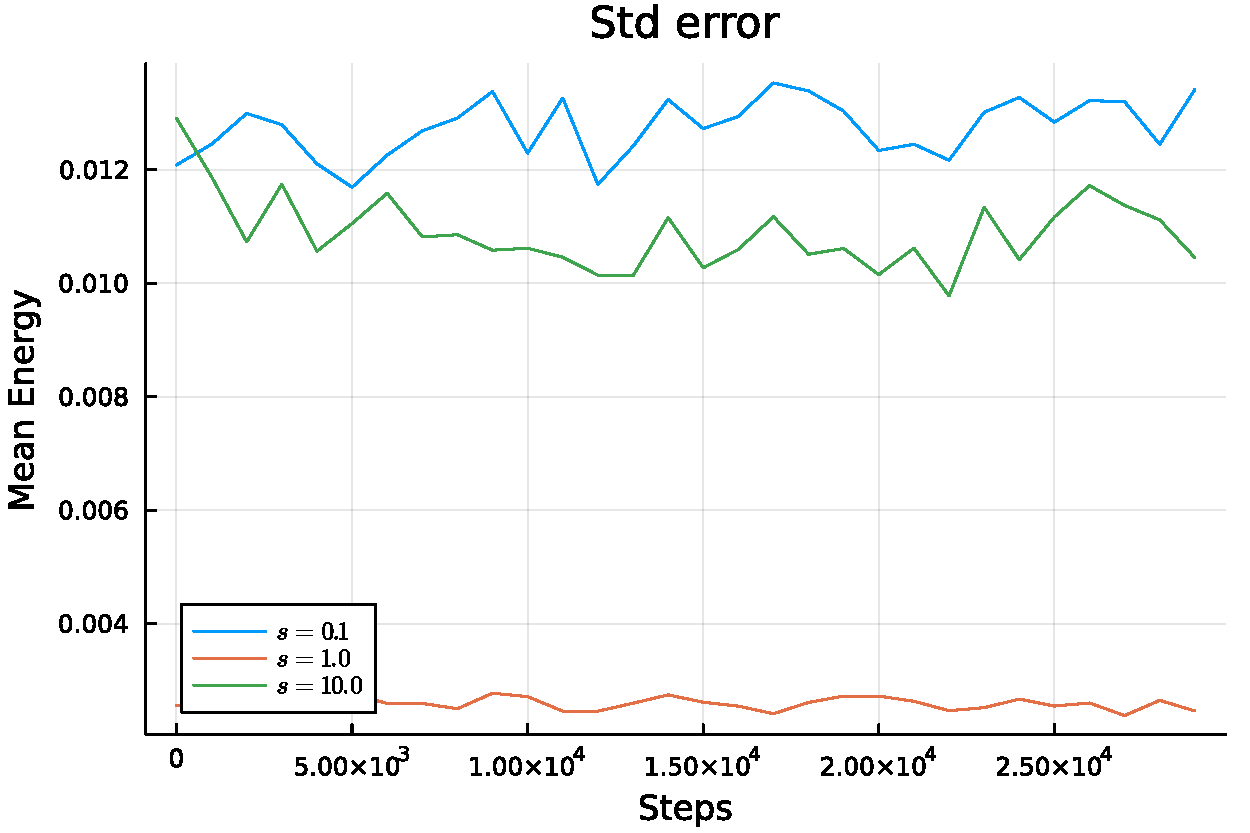
\includegraphics[width=\textwidth]{../saves/task1a.stds.pdf}
		\caption{Stds}
		% \label{fig:three sin x}
	\end{subfigure}
	\caption{Finding a good step size $s$}
	\label{fig:find_a}
\end{figure}

\subsection{Approximating equilibration time}

To observe the ground state energy properly, the simulation needs time to equilibrate, as it starts from random initial conditions. To find the equilibration time we vary over a few $s$ values. The results are displayed in \autoref{fig:equi}

\begin{figure}[H]
	\begin{subfigure}[b]{0.49\textwidth}
		\centering
		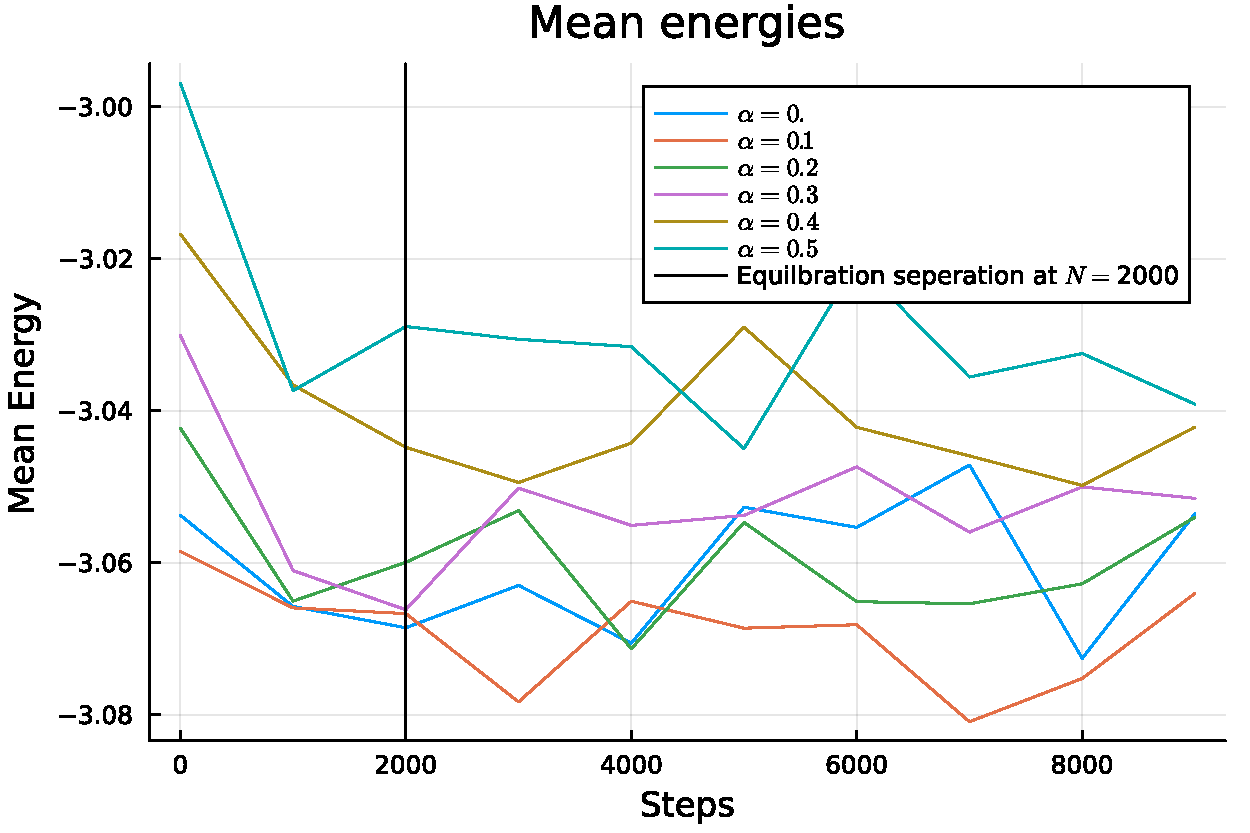
\includegraphics[width=\textwidth]{../saves/task1b.energies.pdf}
		\caption{Energies}
		% \label{fig:three sin x}
	\end{subfigure}
	\hfill
	\begin{subfigure}[b]{0.49\textwidth}
		\centering
		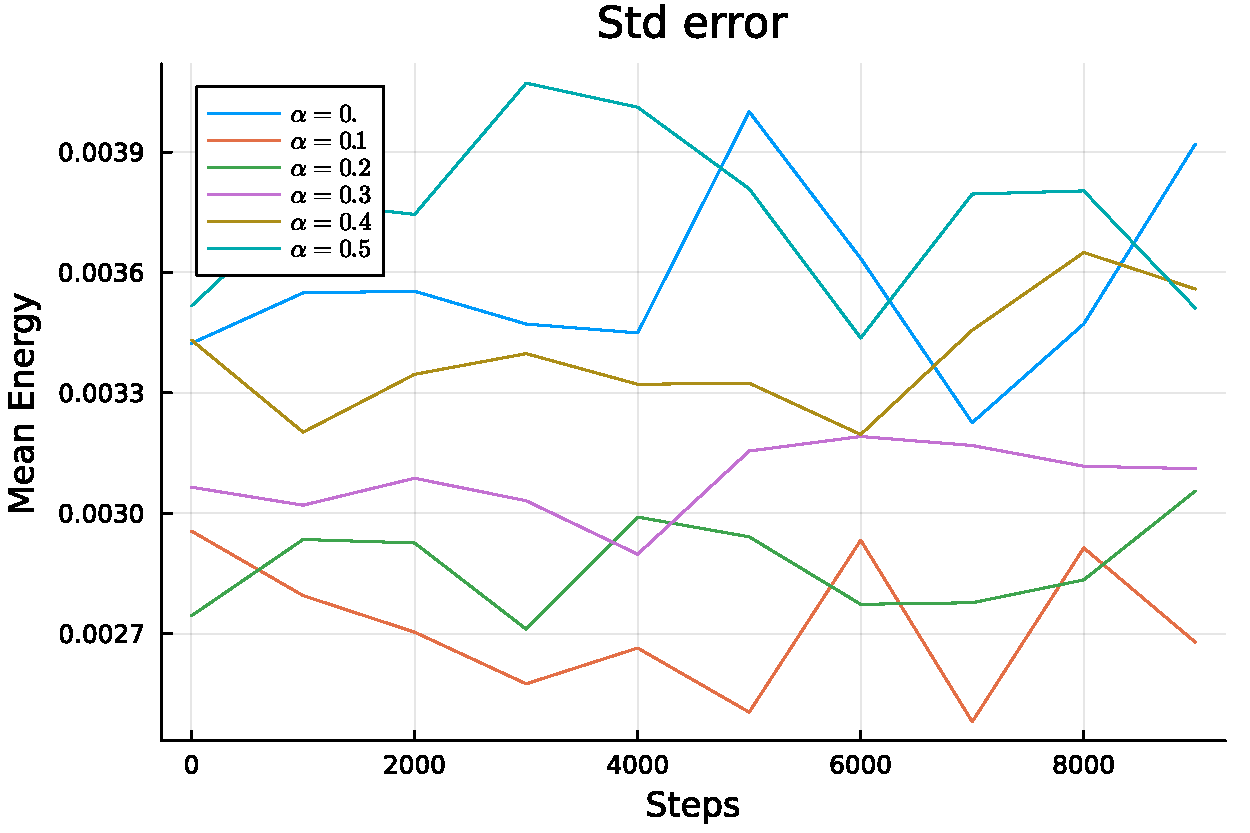
\includegraphics[width=\textwidth]{../saves/task1b.stds.pdf}
		\caption{Stds}
		% \label{fig:three sin x}
	\end{subfigure}
	\caption{Found equilibration time with 2000 steps}
	\label{fig:equi}
\end{figure}

\subsection{Investigate variational parameter $\alpha$}

Now we can stat finding the optimal trial wave function and corresponding minimal energy. For the optimal $\alpha$ I get $\alpha=0.16$, for the optimal $\kappa=1.93$ The results are displayed in \autoref{fig:optalpha} and \autoref{fig:optkappa} respectively. The respective energy minima are quoted in the figures, they are the same in the range of their respective 1-sigma deviation.

\begin{figure}[H]
	\begin{subfigure}[b]{0.49\textwidth}
		\centering
		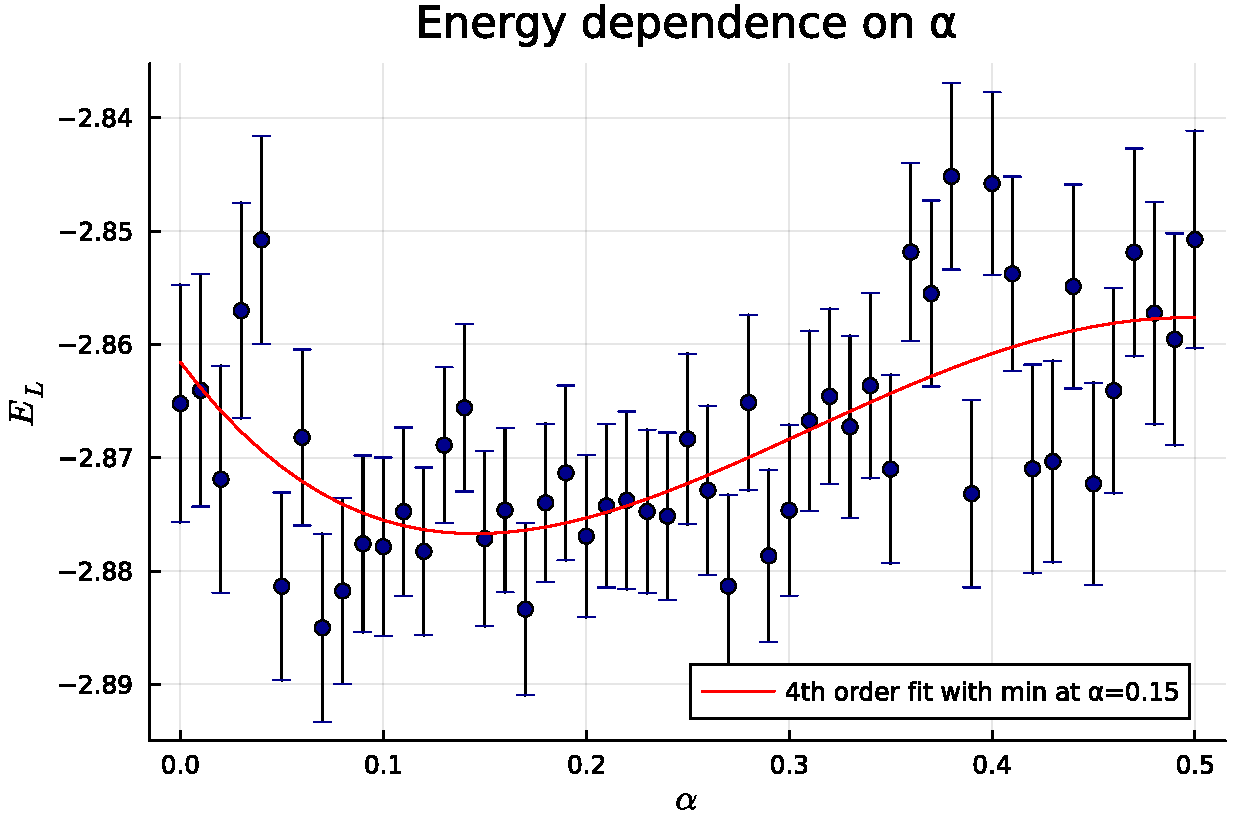
\includegraphics[width=\textwidth]{../saves/task1c.avEnergies.pdf}
		\caption{Energies}
		% \label{fig:three sin x}
	\end{subfigure}
	\hfill
	\begin{subfigure}[b]{0.49\textwidth}
		\centering
		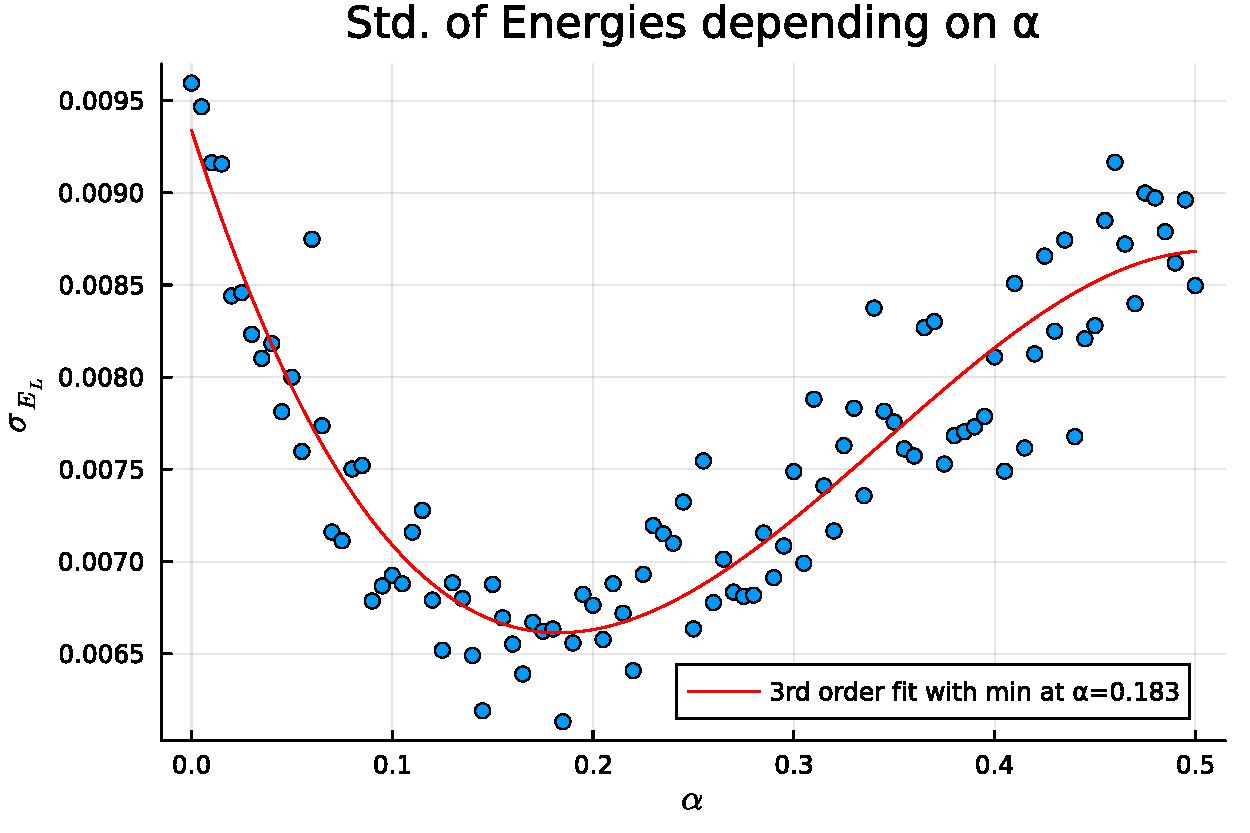
\includegraphics[width=\textwidth]{../saves/task1c.avStd.pdf}
		\caption{Stds}
		% \label{fig:three sin x}
	\end{subfigure}
	\caption{Finding optimal $\alpha=0.16$}
	\label{fig:optalpha}
\end{figure}

\subsection{Investigate variational Parameter $\kappa$}

\begin{figure}[H]
	\begin{subfigure}[b]{0.49\textwidth}
		\centering
		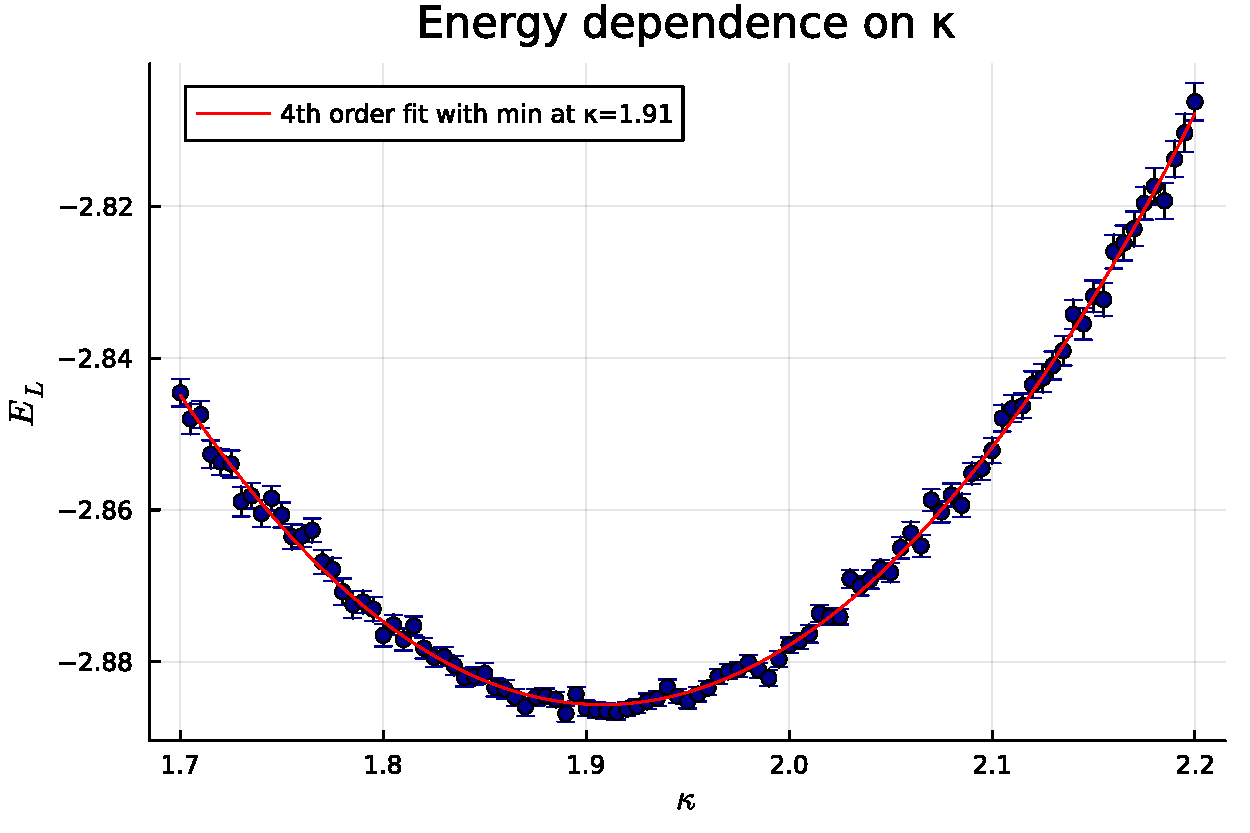
\includegraphics[width=\textwidth]{../saves/task1d.avEnergies.pdf}
		\caption{Energies}
		% \label{fig:three sin x}
	\end{subfigure}
	\hfill
	\begin{subfigure}[b]{0.49\textwidth}
		\centering
		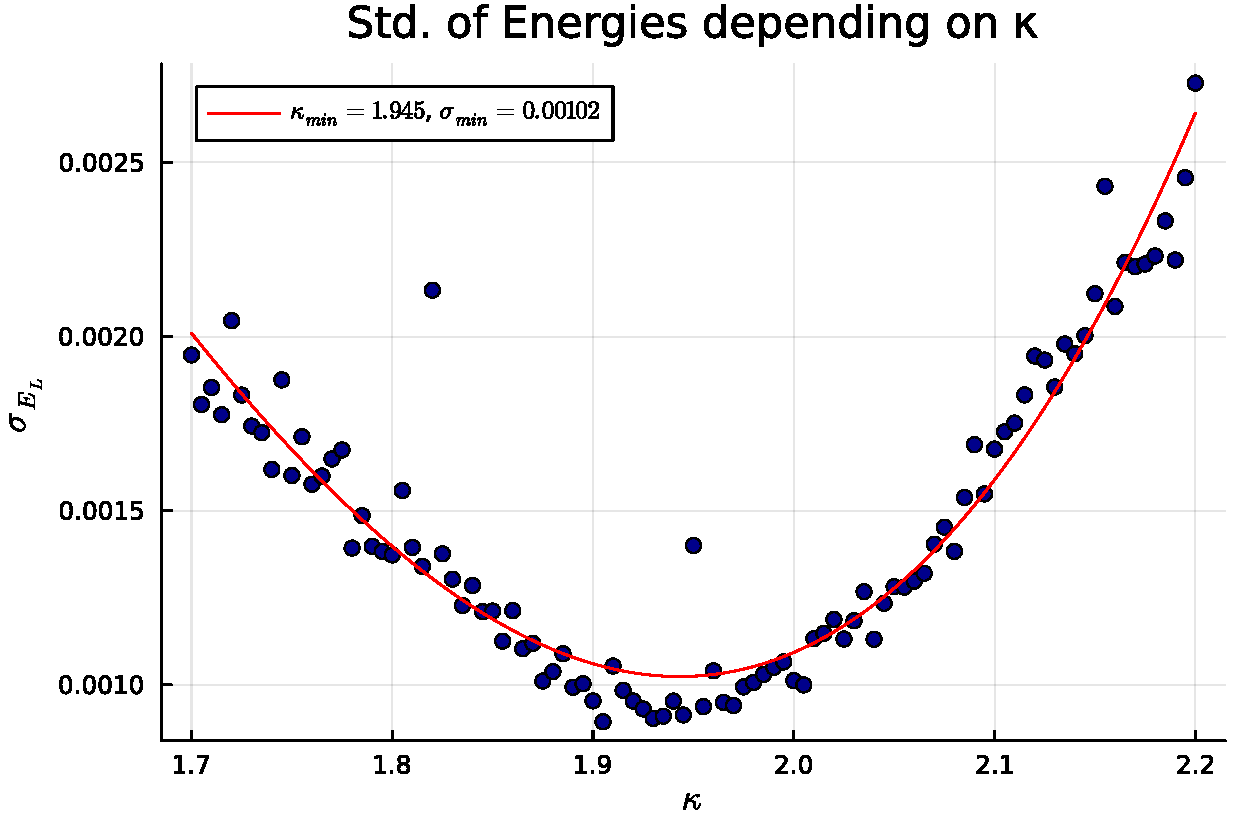
\includegraphics[width=\textwidth]{../saves/task1d.avStd.pdf}
		\caption{Stds}
		% \label{fig:three sin x}
	\end{subfigure}
	\caption{Finding optimal $\kappa=1.93$}
	\label{fig:optkappa}
\end{figure}

\subsection{Optimizing parameters $\alpha$, $\beta$ and $\kappa$}

When running an optimization over all three parameters at the same time I get:

\begin{table}[H]
	\centering
	\begin{tabular}{|c|c|c|c|c|} 
	\hline
		& $\alpha$ & $\beta$ & $\kappa$ & $E_L$ \\
	\hline
		Optimized &  &  &  &  \\ 
	 	Run with given & 0.18 & 0.38 & 1.85 & -2.892$\pm$0.002 \\
	\hline 
		Experimental &  &  &  & -2.90338583(13) \\ 
	\hline
\end{tabular}
	\caption{Finding the optimal trial wave function parameters.}
	\label{tab:optimparams}
\end{table}

\section{Variational Monte Carlo with Fokker-Plank support}

\subsection{Quantum force}

Given the trial wave function 
\begin{align*}
	\psi_T = e^{-\kappa r_1}e^{-\kappa r_2}e^{\frac{\beta r_{12}}{1+\alpha r_{12}}}
\end{align*}
The corresponding quantum force follows
\begin{align*}
	\Vec F (R) &=  \frac{\nabla \rho}{\rho} = 2\frac{\nabla \psi_T}{\psi_T}.
\end{align*}

As the trial wave function consist of exp-functions I will only consider $\nabla \Psi_T$ and cancel the $\Psi_T$ terms afterwards.

\begin{align*}
	2 \nabla \Psi_{T} = -2 \left (
	\begin{matrix}
		\frac{\kappa}{r_1} \Vec{r}_1 + \beta (\frac{u}{r_{12}} - \frac{\alpha}{u^2}) \cdot (\Vec r_1- \Vec r_2) \\
		\frac{\kappa}{r_2} \Vec{r}_1 - \beta (\frac{u}{r_{12}} - \frac{\alpha}{u^2}) \cdot (\Vec r_1- \Vec r_2)
	\end{matrix} \right ) \Psi_T, = \frac{\Vec F (R)}{\Psi_T}
\end{align*}

where $u = 1+\alpha r_{12}$, $r_1 = |\Vec r_1|$, $r_2 = |\Vec r_2|$ and $r_{12} = |\Vec r_1 - \Vec r_2|$.

\subsection{Investigate variational parameter $\Delta\tau$}

Investigating the parameter $\Delta \tau$ for four different values revelas thath the best of these is $\Delta \tau=0.05$ as $E_L=-2.895$. As expected is this result closer to the experimental value than solely using VMC.

\begin{figure}[H]
	\begin{subfigure}[b]{0.49\textwidth}
		\centering
		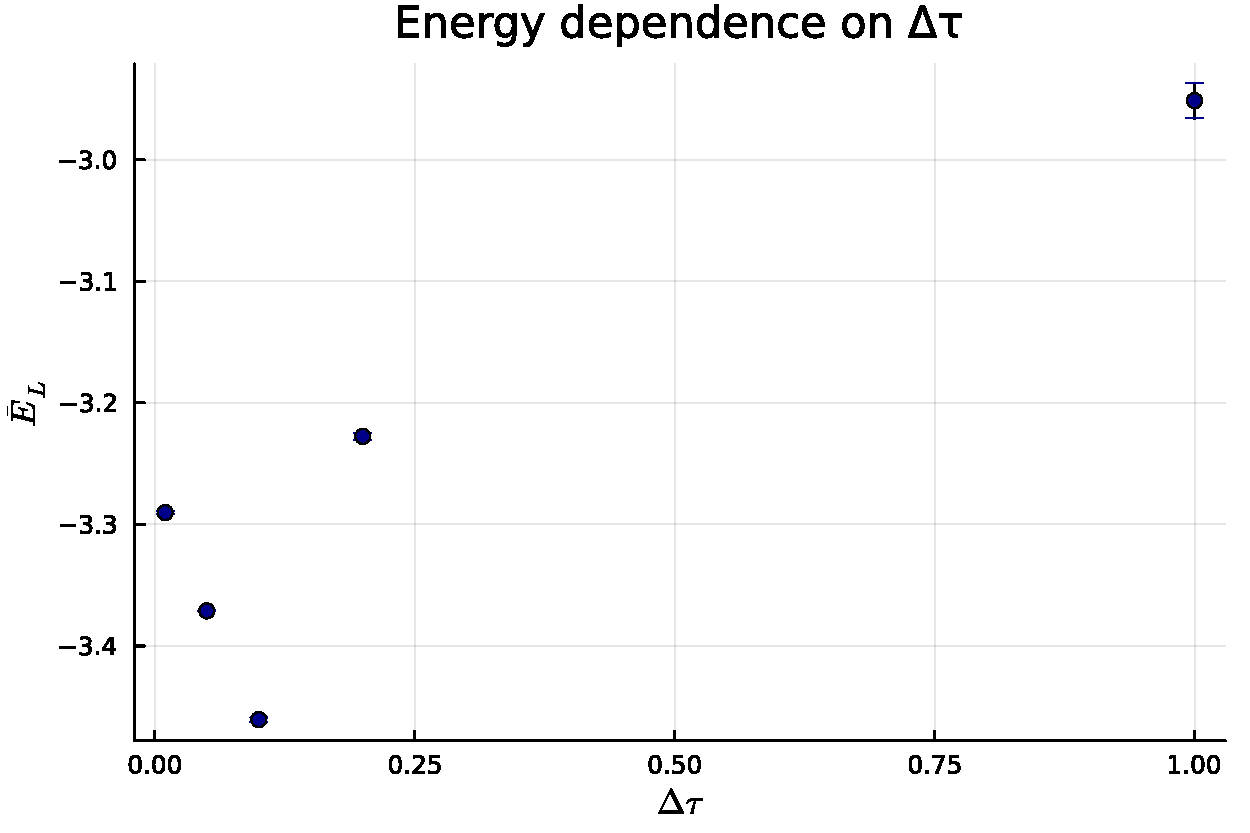
\includegraphics[width=\textwidth]{../saves/task1g.avEnergies.pdf}
		\caption{Energies}
		% \label{fig:three sin x}
	\end{subfigure}
	\hfill
	\begin{subfigure}[b]{0.49\textwidth}
		\centering
		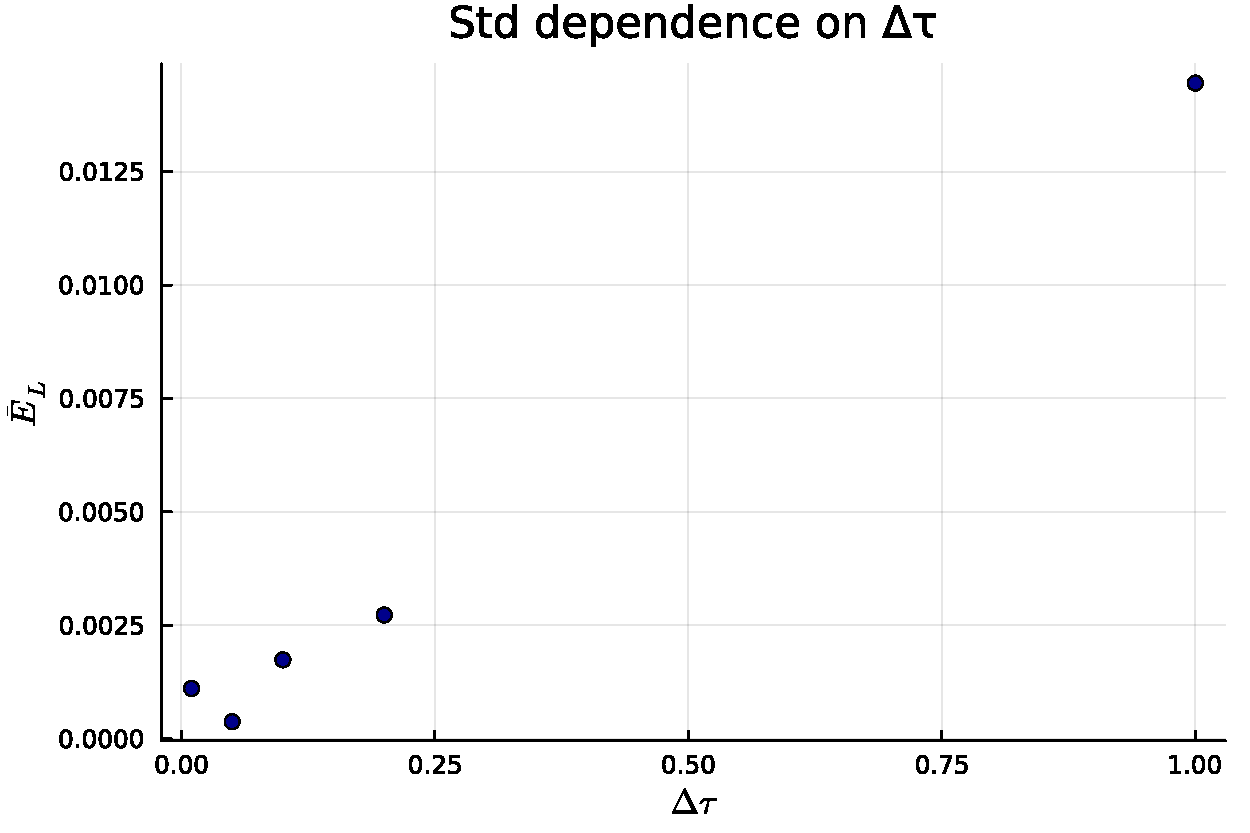
\includegraphics[width=\textwidth]{../saves/task1g.avStd.pdf}
		\caption{Stds}
		% \label{fig:three sin x}
	\end{subfigure}
\end{figure}

\subsection{Electron density}

The Electron density, displayed in \autoref{fig:densityFP} after equilibration follows a gaussian distribution with mean $\mu=0.76$. This could be interpreted as the first orbit of the helium atom, where both electrons are located.

\begin{figure}[H]
	\centering
	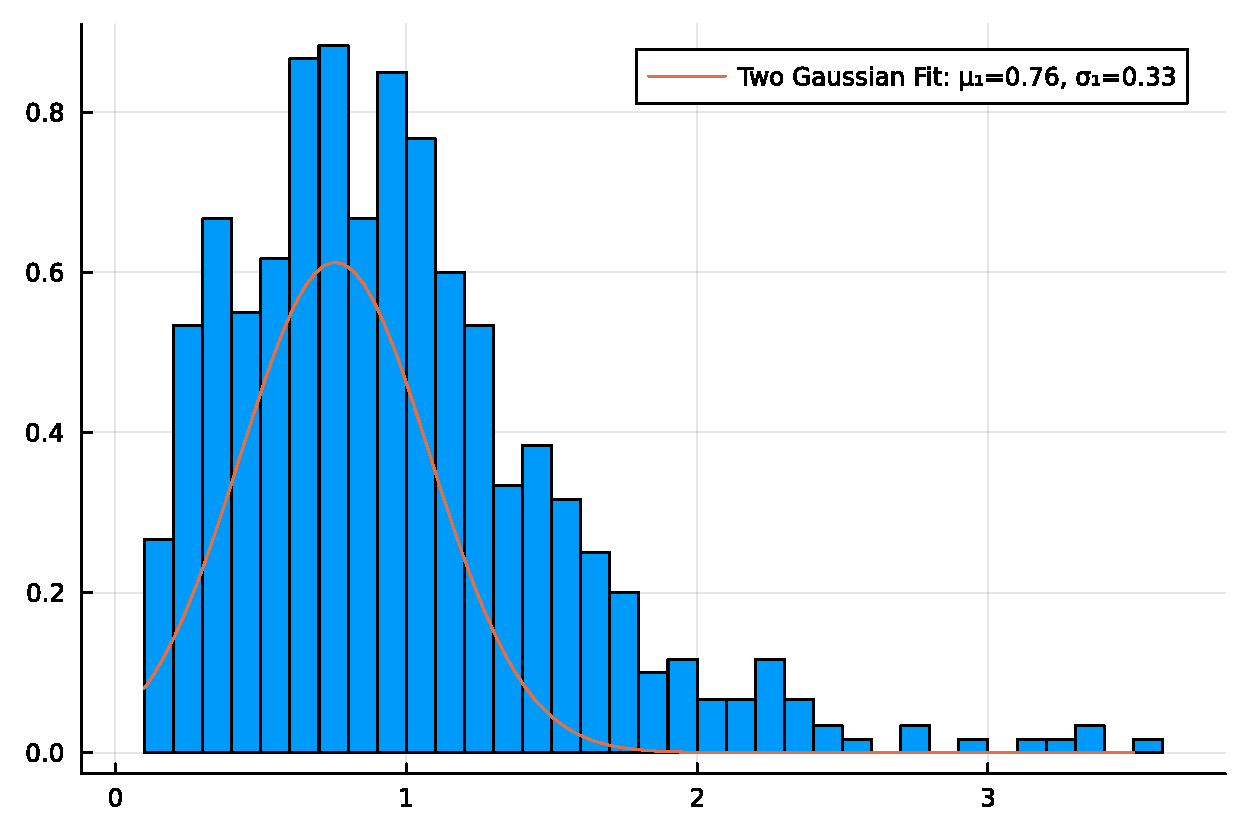
\includegraphics[width=\textwidth]{../saves/task1h.density.pdf}
	\caption{Electron density}
	\label{fig:densityFP}
\end{figure}

\section{Diffusion Monte Carlo simulation of a Helium atom}

One would use Diffusion Monte Carlo, because it can lead to arbitrary accurate results, given the right loss function. Normaly one uses it after a rough estimate with VMC to get closer to the exact result. \\
Unfortunately, the Diffusion Monte-Carlo does not converge to the experimental value, as displayed in \autoref{fig:DMC}. Also the electron density gives qualitatively not the same as in VMC, as displayed in \autoref{fig:densityDMC}. This indicates a bug, my code can be found under https://github.com/simonblaue/MCP-Ex5.git. 

\begin{figure}[H]
	\centering
	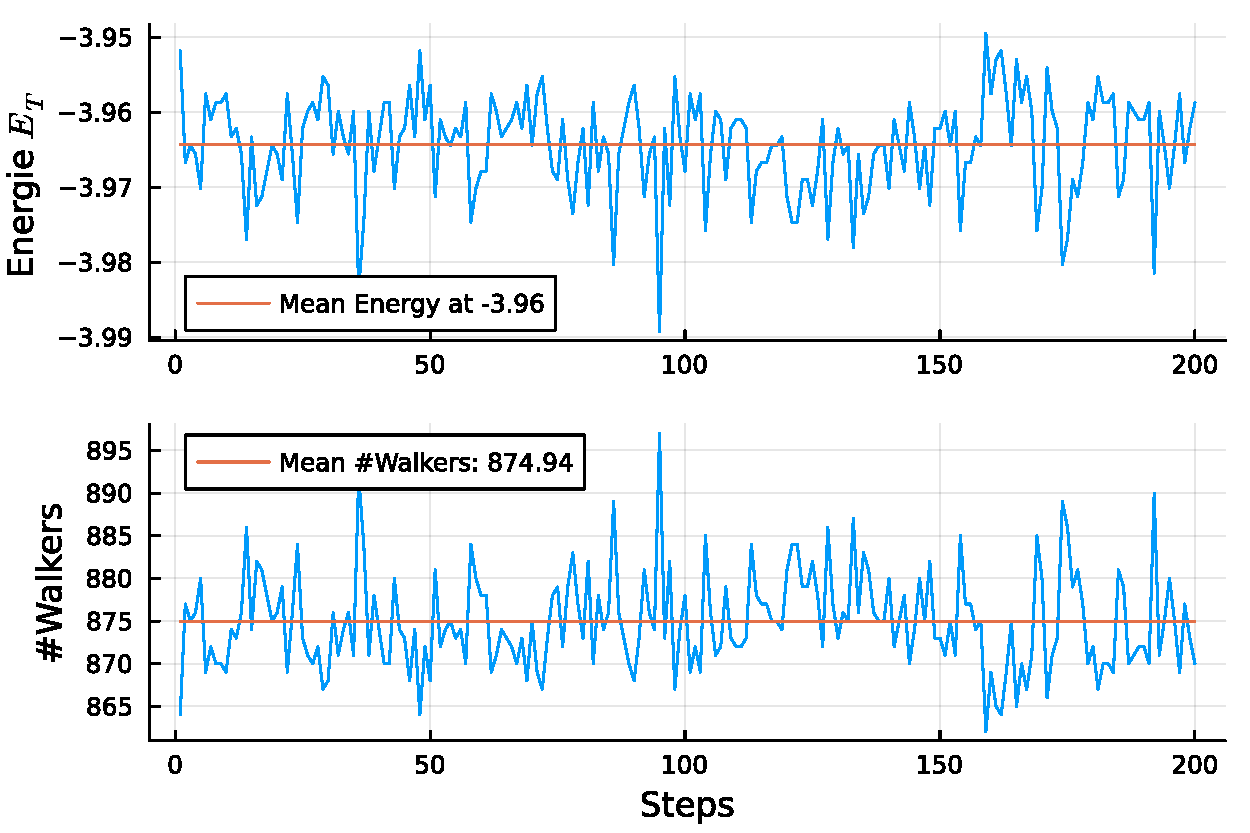
\includegraphics[width=\textwidth]{../saves/task2b.Energies.pdf}
	\caption{Energy $E_T$ and number of walkers, plotted for every 100th step. In total the simulation run for 20000 steps.}
	\label{fig:DMC}
\end{figure}

\begin{figure}[H]
	\centering
	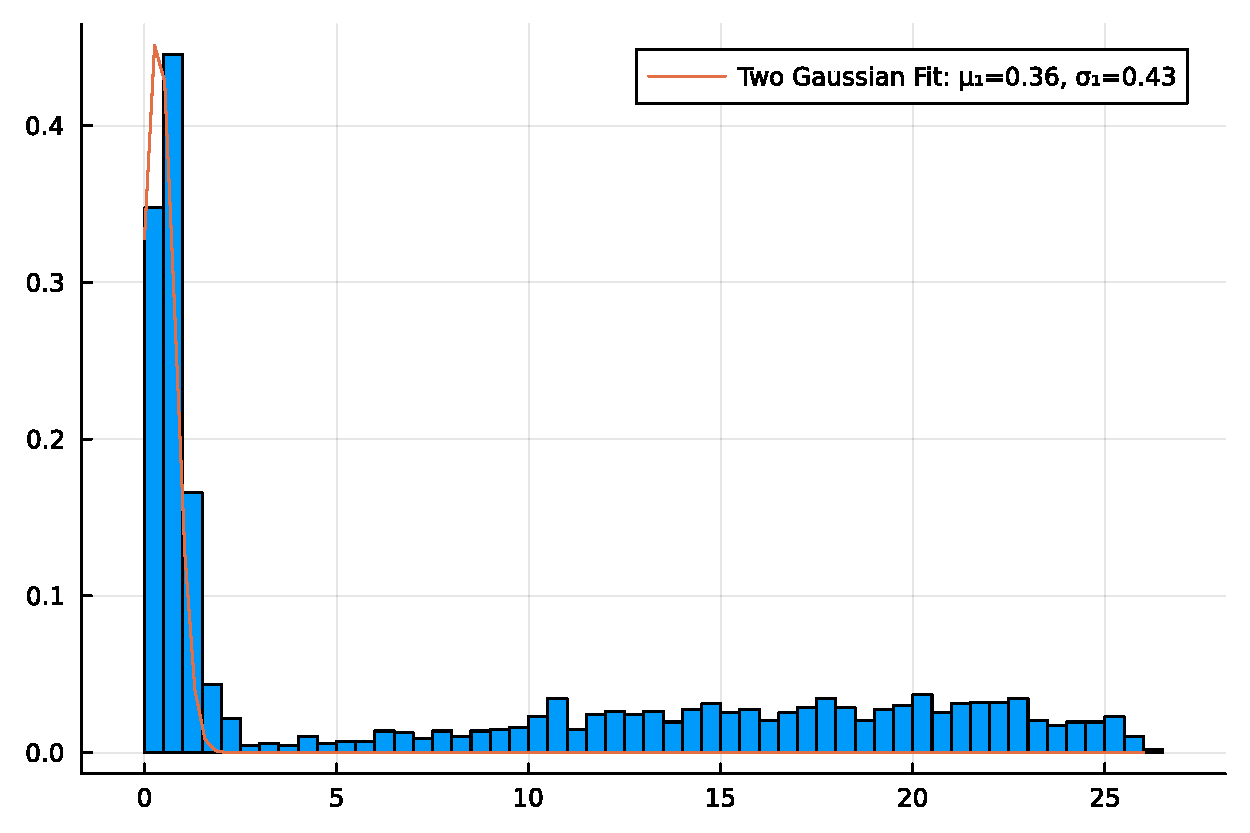
\includegraphics[width=\textwidth]{../saves/task2b.density.pdf}
	\caption{Electron density for DMC}
	\label{fig:densityDMC}
\end{figure}

\section{Feynman Path Integral Quantum Mechanics}


The energy and squared wave function for the 1d oscillator are displayed in \autoref{fig:harmon1d}. The viral theorem does not hold as the kinetic energy dominates. The histogram corresponds to the likelihood of the positions, thus the probability density and the squared wave function. \\
The same is true for the 2d case, only now does the kinetic energy not dominate as much as before. The result for 2d is displayed in \autoref{fig:harmon2d}.

\subsection{One dimensional harmonic oscillator}


\begin{figure}[H]
	\begin{subfigure}[b]{0.49\textwidth}
		\centering
		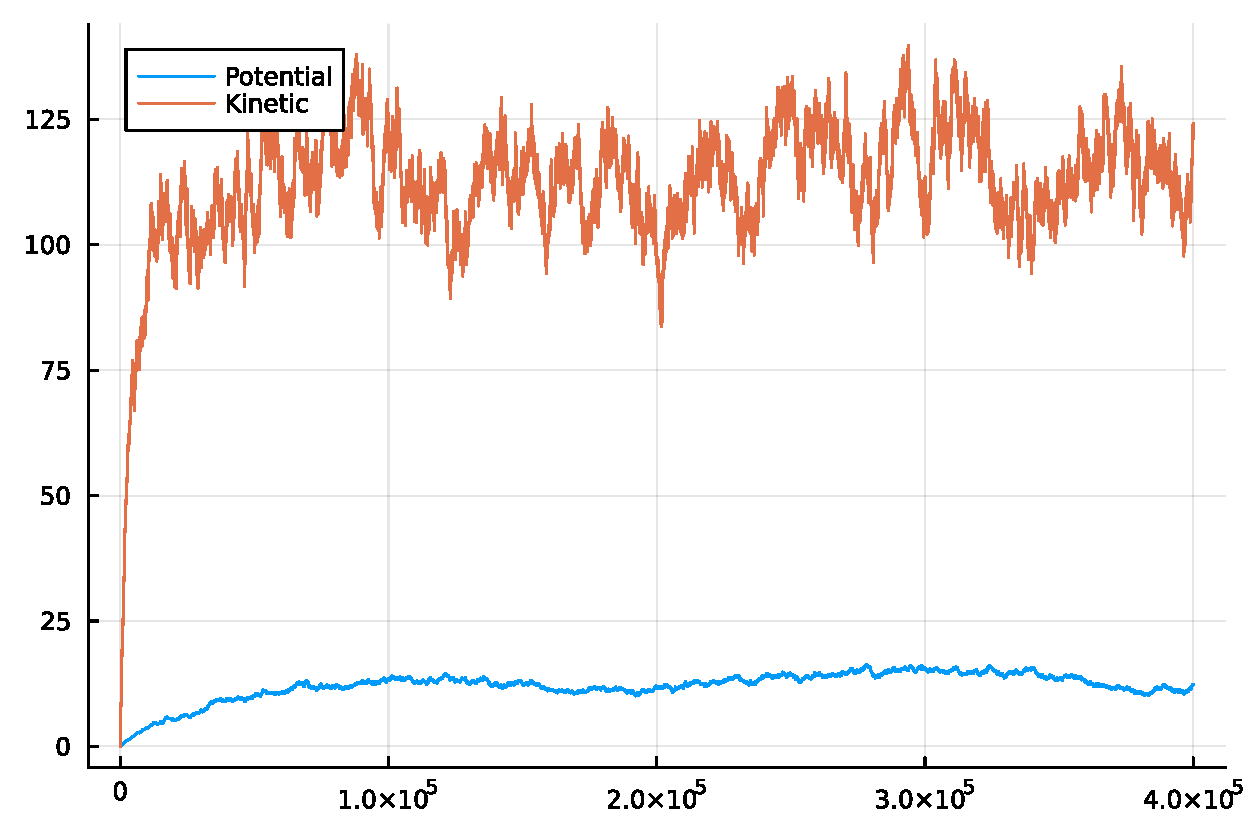
\includegraphics[width=\textwidth]{../saves/task3a.energies.pdf}
		\caption{Energies}
		% \label{fig:three sin x}
	\end{subfigure}
	\hfill
	\begin{subfigure}[b]{0.49\textwidth}
		\centering
		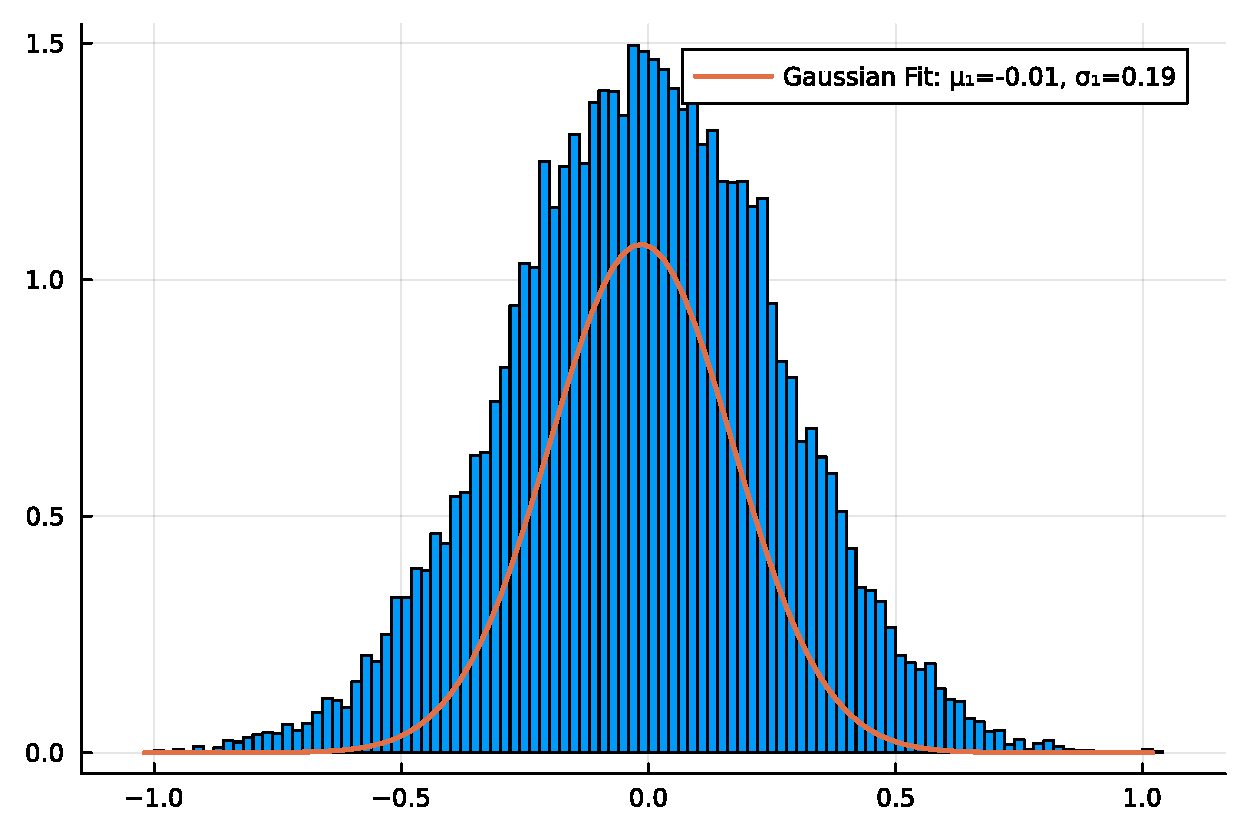
\includegraphics[width=\textwidth]{../saves/task3b.hist.pdf}
		\caption{quared wave function}
		% \label{fig:three sin x}
	\end{subfigure}
	\caption{1D Oszillator}
	\label{fig:harmon1d}
\end{figure}


\subsection{Two dimensional harmonic oscillator}

\begin{figure}[H]
	\begin{subfigure}[b]{0.49\textwidth}
		\centering
		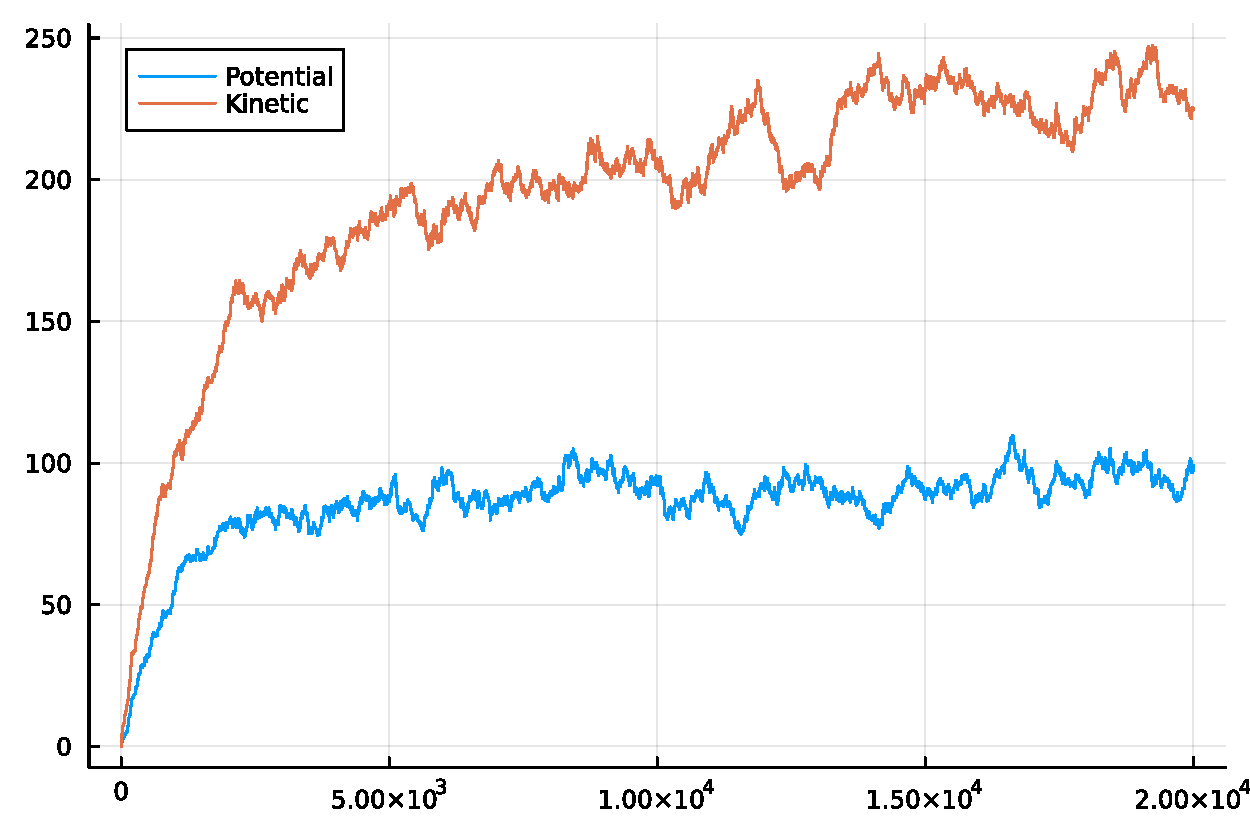
\includegraphics[width=\textwidth]{../saves/task3c.energies.pdf}
		\caption{Energies}
		% \label{fig:three sin x}
	\end{subfigure}
	\hfill
	\begin{subfigure}[b]{0.49\textwidth}
		\centering
		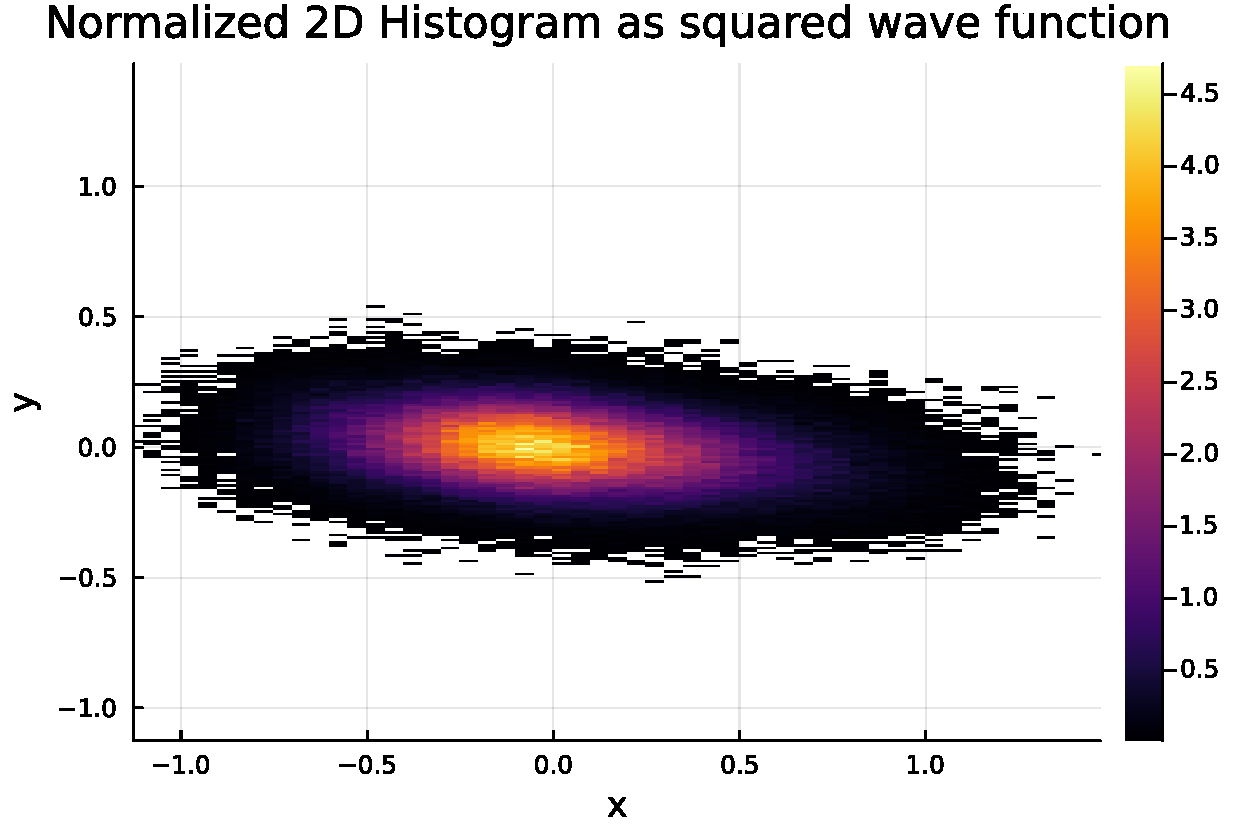
\includegraphics[width=\textwidth]{../saves/task3c.hist.pdf}
		\caption{Squared wave function}
		% \label{fig:three sin x}
	\end{subfigure}
	\caption{2D Oszillator}
	\label{fig:harmon2d}
\end{figure}

%----------------------------------------------------------------------------------------
%	DISCUSSION
%----------------------------------------------------------------------------------------

% \section{Discussion}

%----------------------------------------------------------------------------------------
%	BIBLIOGRAPHY
%----------------------------------------------------------------------------------------
\newpage

\printbibliography % Output the bibliography

%----------------------------------------------------------------------------------------

\end{document}